%%%%%%%%%%%%%%%%%%%%%%%%%%%%%%%%%%%%%%%%%
% Short Sectioned Assignment LaTeX Template Version 1.0 (5/5/12)
% This template has been downloaded from: http://www.LaTeXTemplates.com
% Original author:  Frits Wenneker (http://www.howtotex.com)
% License: CC BY-NC-SA 3.0 (http://creativecommons.org/licenses/by-nc-sa/3.0/)
%%%%%%%%%%%%%%%%%%%%%%%%%%%%%%%%%%%%%%%%%

%----------------------------------------------------------------------------------------
%	PACKAGES AND OTHER DOCUMENT CONFIGURATIONS
%----------------------------------------------------------------------------------------

\documentclass[paper=a4, fontsize=11pt]{scrartcl} % A4 paper and 11pt font size

% ---- Entrada y salida de texto -----

\usepackage[T1]{fontenc} % Use 8-bit encoding that has 256 glyphs
\usepackage[utf8]{inputenc}
%\usepackage{fourier} % Use the Adobe Utopia font for the document - comment this line to return to the LaTeX default

% ---- Idioma --------

\usepackage[spanish, es-tabla]{babel} % Selecciona el español para palabras introducidas automáticamente, p.ej. "septiembre" en la fecha y especifica que se use la palabra Tabla en vez de Cuadro

% ---- Otros paquetes ----

\usepackage{url} % ,href} %para incluir URLs e hipervínculos dentro del texto (aunque hay que instalar href)
\usepackage{amsmath,amsfonts,amsthm} % Math packages
%\usepackage{graphics,graphicx, floatrow} %para incluir imágenes y notas en las imágenes
\usepackage{graphics,graphicx, float} %para incluir imágenes y colocarlas

% Para hacer tablas comlejas
%\usepackage{multirow}
%\usepackage{threeparttable}

%\usepackage{sectsty} % Allows customizing section commands
%\allsectionsfont{\centering \normalfont\scshape} % Make all sections centered, the default font and small caps

\usepackage{fancyhdr} % Custom headers and footers
\pagestyle{fancyplain} % Makes all pages in the document conform to the custom headers and footers
\usepackage{eurosym} % Para poder añadir el símbolo del euro
\fancyhead{} % No page header - if you want one, create it in the same way as the footers below
\fancyfoot[L]{} % Empty left footer
\fancyfoot[C]{} % Empty center footer
\fancyfoot[R]{\thepage} % Page numbering for right footer
\renewcommand{\headrulewidth}{0pt} % Remove header underlines
\renewcommand{\footrulewidth}{0pt} % Remove footer underlines
\setlength{\headheight}{13.6pt} % Customize the height of the header

\numberwithin{equation}{section} % Number equations within sections (i.e. 1.1, 1.2, 2.1, 2.2 instead of 1, 2, 3, 4)
%\numberwithin{figure}{section} % Number figures within sections (i.e. 1.1, 1.2, 2.1, 2.2 instead of 1, 2, 3, 4)
%\numberwithin{table}{section} % Number tables within sections (i.e. 1.1, 1.2, 2.1, 2.2 instead of 1, 2, 3, 4)

\setlength\parindent{0pt} % Removes all indentation from paragraphs - comment this line for an assignment with lots of text

\newcommand{\horrule}[1]{\rule{\linewidth}{#1}} % Create horizontal rule command with 1 argument of height

% Margins
\usepackage[margin=1.25in]{geometry}

% Begin section numbering at 0
\setcounter{section}{-1} 

% Hyperlinks
\usepackage{hyperref, xcolor}
\hypersetup{
  % hidelinks = true,   % Oculta todos los enlaces.
  colorlinks = true,   % Muestra todos los enlaces, sin bordes alrededor.
  linkcolor={black},     % Color de enlaces genéricos
  citecolor={black},   % Color de enlaces de referencias
  urlcolor={magenta}     % Color de enlaces de URL
}
  % Configuración del documento

%----------------------------------------------------------------------------------------
%	TÍTULO Y DATOS DE LOS ALUMNOS
%----------------------------------------------------------------------------------------

\title{	
	\normalfont \normalsize 
	\textsc{\textbf{Fundamentos de Redes (2017-2018)} \\ Doble Grado en Ingeniería Informática y Matemáticas \\ Universidad de Granada} \\ [25pt] 
	\horrule{0.5pt} \\[0.4cm]
	\huge Invisible Internet Project (I2P) \\ 
	\horrule{2pt} \\[0.5cm] 
}

\author{Antonio Coín Castro \\ Alberto Jesús Durán López} 
\date{\normalsize\today}

%----------------------------------------------------------------------------------------
% DOCUMENTOg
%----------------------------------------------------------------------------------------

\begin{document}
	\maketitle       % título
	\newpage 
	\tableofcontents % índice
	\newpage
	
	
	
	
	\section{Motivación}
	
	El incremento en el uso cotidiano de las nuevas tecnologías conlleva una serie de riesgos ocultos a la mayoría de los usuarios, que normalmente no son conscientes de los mismos, sino que se centran en el uso de las mismas sin preocuparse de otros factores.\\
	
	Es por esto que vemos de vital importancia poner de manifiesto los puntos negativos que afectan a los usuarios de Internet, sobre todo en cuanto a privacidad se refiere. Este problema en particular es preocupante, pues cada vez que nos conectamos a la red cedemos una gran cantidad de datos que en manos equivocadas pueden suponer un grave peligro para nosotros.\\
	
	Afortunadamente, existen diversos métodos que, en mayor o menor medida, nos ayudan a prevenir esta cesión indiscriminada de datos, sin privarnos de la facilidad y comodidad del uso corriente de Internet. En este trabajo nos centraremos en un software en particular, llamado \textbf{Invisible Internet Project (I2P)}, y también hablaremos en general sobre redes de anonimato. Sin embargo, antes explicaremos con un poco más de detalle los riesgos concretos en un acceso corriente a Internet, así como otros métodos menos sofisticados para protegernos.
	
	
	
	
	\section{Anonimato en el acceso corriente a Internet}
	
	¿Alguna vez te has planteado qué ocurre cuando abres el navegador y te conectas a una web de Internet? En teoría es un proceso sencillo de cara al usuario, algo que hacemos de forma casi automática. Sin embargo, lo que en realidad ocurre en las capas interiores es un proceso complejo, y tratando de entenderlo podemos condicionar nuestro comportamiento en la red para intentar proteger nuestra privacidad.\\
	
	Para ilustrar el proceso de conexión de forma muy simplificada, podemos pensar en una plaza o un parque de una ciudad, y personas entrando y saliendo del mismo. No es extraño pensar que al conectarnos a Internet realizamos un proceso análogo a entrar en la plaza, pues podemos ver que hay otros usuarios conectados, y relacionarnos con ellos si así lo queremos. Pero no en realidad no es exactamente lo mismo, pues en el primer caso somos conscientes de los riesgos que conlleva entrar al parque, y solo compartimos la información que nosotros queremos en cada momento. En Internet, automáticamente estamos cediendo una gran cantidad de información, como si fueramos al parque con una hoja con nuestros datos personales en alto, y cualquier persona pudiera, desde la distancia, saber a qué nos dedicamos, por qué hemos venido al parque, nuestra dirección, etc.\\
	
	Uno de los mayores problemas es la huella digital que dejamos inconscientemente al realizar cualquier conexión, compuesta por diferentes elemntos que pueden ser potencialmente usados para identificarnos. Un elemento destacable es nuestra \textit{dirección IP}, la cual es fácilmente detectable y nos identifica de forma unívoca en Internet. Además, es posible \textbf{geolocalizar} el dispositivo desde el cual se está accediendo, simplemente con saber la dirección IP (por ejemplo, en \href{https://whatismyipaddress.com/}{\url{what is my ip address}}).\\
	
	
	Es cierto que mucha gente se conecta a Internet con una IP temporal asignada para una sola sesión. Sin embargo, dichas direcciones son registradas por los proveedores de servicio (\textit{ISP}), por lo que sería posible descubrir quién usó una cierta dirección IP en un intervalo tiempo concreto.\\
	
	Existen otros problemas derivados, como el envío del historial de búsqueda, cookies de rastreo, y otra información almacenada en nuestro navegador que nos puede identificar en la red. En general, compartir esta información no tiene por qué ser dañino para nosotros, pero en un entorno tan grande como Internet, toda precaución es buena. 
	
	
	
	
	\section{Métodos para mantener el anonimato}
	
	A la hora de ocultar nuestro rastro en Internet existen diferentes alternativas, con diferentes niveles de efectividad.
	
\subsection{Proxy} Se trata de un servidor intermediario entre las conexiones de un cliente y un servidor, centrado en la navegación. De esta manera, al visitar una página web se puede enviar y recibir información a través de un proxy, y así ocultar nuestra dirección IP a la página de destino, que verá la IP del proxy. Puede utilizarse para acceder a contenido bloqueado en algunos países, como medio de evitar la censura.

\subsection{VPN} Es un acrónimo para \textit{Virtual Private Network}, red privada virtual. Se trata de un medio de extender una red privada a través de una red pública, de forma que simula que un usuario conectado a través de VPN forme parte físicamente de la red privada. Esto proporciona diversas ventajas:

\begin{itemize}
	\item Se puede acceder remotamente a los recursos de la red privada como si se formase parte de ella.
	\item Se camufla la dirección IP, pues la dirección que se ve es aquella que proporciona la red virtual.
	\item Se garantiza la confidencialidad, de forma que los paquetes intercambiados en la red están encriptados.
	\item Existe un sistema de autentificación para conectarse a la red e impedir accesos no deseados.
	\item También se proporcionan mecanismos para mantener la integridad de los mensajes y detectar mensajes fraudulentos.
\end{itemize}
	
\subsection{Redes de anonimato} 

Una red de anonimato permite a los usuarios acceder a la web de forma que se intenta bloquear cualquier seguimiento de su identidad en Internet. Para ello, se canaliza el tráfico a través de una red global de servidores voluntarios.\\

Son el objetivo central de este trabajo, y las discutiremos con detalle posteriormente.

\subsection{Otros} Existen otros mecanismos, menos sofisticados pero muchas veces muy efectivos, como por ejemplo utilizar buscadores que respetan la privacidad (\href{https://duckduckgo.com/}{\url{DuckDuckGo}}).




    \section{Invisible Internet Project. Estructura, funcionamiento y seguridad}

I2P es una herramienta de \textbf{software libre} que ofrece una capa de red de abstracción  \textbf{distribuida} para comunicaciones entre ordenadores, la cual permite a las aplicaciones que la utilizan transmitir mensajes de forma anónima y segura. Se trata de una red superpuesta (del inglés \textit{overlay network}), que funciona con nodos virtuales en una red construida sobre Internet, cuyas conexiones en la red subyacente pueden ser estar ubicadas en zonas geográficamente muy alejadas. Su misión es conseguir que los datos lleguen desde el origen al destino aunque no exista una conexión directa entre los nodos.\\

En este caso, la selección de ruta o \textit{routing} que ofrece I2P se basa en una serie de nodos conectados a la misma red, que crean caminos temporales y unidireccionales (túneles), siguiendo la técnica de enrutamiento \textit{garlic}, que veremos a más adelante\\

Además, todas las comunicaciones están encriptadas \textit{punto a punto}, lo que añade una capa extra de seguridad a nuestras aplicaciones.

\subsection{Nodos y túneles}

En la terminología de \textit{I2P}, el software que implementa la capa de red se denomina \textbf{router}, y un ordenador ejecutándolo se denomina \textbf{nodo}. Para garantizar que los mensajes enviados sean anónimos, se construye para cada cliente una serie de \textit{túneles} de llegada y de salida. Estos túneles son una secuencia de nodos que pasan los mensajes de unos a otros, de manera unidireccional. La red es, por tanto, basada en mensajes, de forma similar al protocolo \textbf{IP}.\\

El mecanismo es el siguiente: cuando un cliente quiere enviar un mensaje a otro cliente, lo pasa a uno de sus nodos de salida que apunta a uno de los nodos de llegada del otro cliente, de forma que después de viajar por el túnel, el mensaje llega a su destino. Cada participante de la red elige la longitud de los túneles, de forma que se alcance un equilibrio entre el anonimato, la latencia y el \textit{throughput} que lo satisfaga. El resultado es que el número de conexiones es el mínimo necesario para satisfacer las necesidades del emisor y del receptor.\\


A la hora de implementar la conexión, la primera vez que un cliente quiere contactar a otro cliente, realizan una consulta a la "base de datos de redes", que es una tabla \textit{hash} distribuida basada en el algoritmo Kademlia, que explicaremos a continuación.\\

Cuando un router I2P quiere contactar con otro router, necesita saber una información mínima, como la \textit{identidad} del router (una clave de encriptación de 2048 bits) o la dirección de contacto donde se encuentra.\\

\begin{figure}
    \centering
	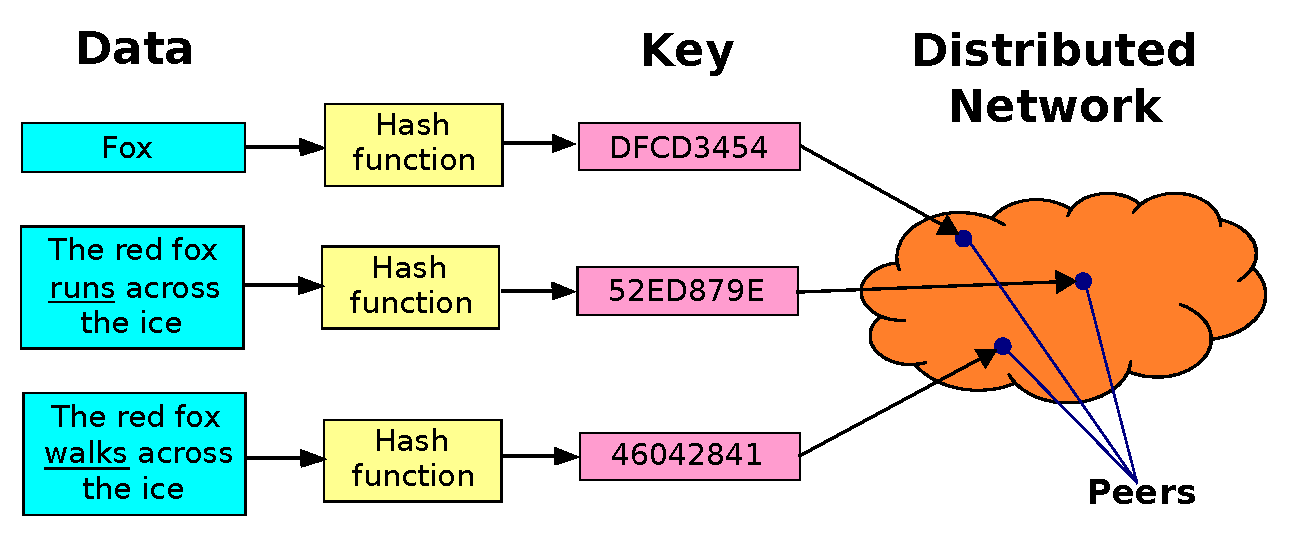
\includegraphics[width=.8\textwidth]{img/DHT}
	\caption{Tabla hash distribuida (DHT)}
\end{figure}


La búsqueda en la tabla se realiza para encontrar de forma eficiente los túneles de entrada del nodo destino, pero los siguientes mensajes entre el emisor y el receptor normalmente incluyen esta información, por lo que no son necesarias nuevas búsquedas.\\

Por último, cabe mencionar que los mensajes enviados entre los routers están definidos por el \textbf{protocolo I2NP}, cuya especificación completa se puede consultar en \cite{I2NP}.

\subsubsection*{Algoritmo Kademlia}


La base de datos de red (\textit{netDB}) se distribuye mediante una técnica simple llamada "\textit{floodfill}", donde un subconjunto de los routers mantienen la base de datos (cada uno tiene una parte). \\

A la hora de realizar una búsqueda desde un nodo, se realiza una consulta al router "floodfill" más cercano. La medida de cercanía se computa siguiendo una modificación del algoritmo Kademlia. Este algoritmo emplea la función XOR entre dos claves de routers para determinar cómo de cerca están uno de otro.\\

La función XOR ($\oplus$) funciona como una \textit{distancia} en el espacio de las claves de los nodos:

\begin{itemize}
	\item La distancia entre un nodo y él mismo es 0.
	\item La distancia es simétrica: $A \ \oplus \ B = B \ \oplus \ A$.
	\item Se verifica la desigualdad triangular: $A \oplus B \leq (A \ \oplus \ C) + (C \ \oplus \ B)$
\end{itemize}

Una red con $2n$ nodos que emplee este algoritmo en su forma más básica necesitará solo $n$ pasos (en el peor caso) para encontrar un nodo en concreto.



\subsection{Enrutamiento tipo \textit{garlic}}

En la tecnología I2P, es necesario comprender qué significa \textit{Garlic}, cuyo término, al no ser preciso, se le puede atribuir a 3 conceptos diferentes: 

\subsubsection*{Cifrado por capas}

En esta técnica se construyen los correspondientes túneles en los que la información, previamente cifrada por el emisor,  viaja a través de una serie de nodos.

Para explicar la comunicación entre 2 usuarios, nos ayudaremos de un pequeño esquema: \\


	
\begin{figure}[h]
	\centering
	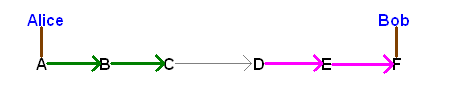
\includegraphics[width=.8\textwidth]{img/alice_bob_tunnel}
	\caption{Comunicación a través de los nodos del túnel}
\end{figure}

Si Alice quiere enviarle un mensaje a Bob, envía el mensaje a uno de sus túneles de salida que está conectado a uno de los túneles de entrada de Bob


El primer nodo del túnel se conoce como \textit{gateway} cuya función es la de fragmentar y empaquetar mensajes I2P en mensajes de túnel de tamaño fijo, que mas adelante son encriptados. 
Los mensajes del túnel están formados por:

\begin{itemize}
	\item ID del tunel: identificadores del tunes de un tamaño de 4 bytes.
	\item Vector de inicializacion de 16 bytes: hace que cada mensaje sea único.
	\item Instrucciones de envío.
	\item Mecanismo de comprobación de errores.
\end{itemize}

Una vez que los mensajes han sido procesados, el \textit{gateway} crea un valor IV aleatorio de 16 bytes, encriptándolo junto al mensaje y enviando al siguiente nodo la tupla \{ID del túnel, IV, mensaje del túnel\}. 

Este proceso es repetido por cada nodo, hasta el nodo final del túnel de salida, que recuperará los datos prepocesados iniciales.



\subsubsection*{Agregación de múltiples mensajes juntos:}
En \textit{Onion Routing} los mensajes se encapsulan en capas de cifrado, a diferencia de \textit{Garlic Routing} que encripta varios mensajes juntos para que el análisis de tráfico realizado por los atacantes resulte más difícil, así como para aumentar la velocidad de transferencia de datos.

\subsubsection*{Cifrado utilizando ElGamal/AES:}
Herramienta para cifrar la información que usa I2P cuyo funcionamiento explicaremos más adelante.




\subsection{Encriptación de la información}

Se trata del mecanismo empleado por cada uno de los routers en cada canal de comunicación para cifrar los paquetes que viajan entre cada uno de ellos, todos los mensajes son cifrados utilizando el algoritmo de cifrado \textit{ElGamal} y posteriormente se utiliza \textit{AES+SessionTag}.\\

Una de las consecuencias más importantes de la encriptación es que, al estar oculto el contenido de los mensajes enviados (la información que se quiere transmitir, y también otros campos necesarios para establecer la comunicación), \textbf{se enmascara la dirección IP del nodo que envía el mensaje}.


\begin{itemize}

\item \textbf{ElGamal:}
Algoritmo de criptografía asimétrica. Su funcionamiento se basa en cálculos sobre logaritmos discretos usando un número primo y dos enteros.   


\item \textbf{AES. :}
Es lo que se conoce como un cifrado simétrico por bloques, es decir, cifra y descifra los datos en bloques de 128 bits cada uno. Para ello utiliza una clave criptográfica específica que puede ser de 128,192 o 256 bits de tamaño. Dicha clave se especifica al nombrar el cifrado usado (AES-128, AES256...). Además, a cada bloque de texto se le aplica una operación XOR con el previo bloque ya cifrado, haciendo cada mensaje único con el uso de un vector de inicialización en el primer bloque. Esto es lo que se conoce como \textit{Cipher Block Chaining - CBC} 


\item \textbf{Algoritmo:} La primera vez que un nodo quiere cifrar un mensaje para otro nodo, ambos cifran las claves para una clave de sesión AES256 con \textit{ElGamal} y se adjuntan los bloques cifrados  AES-256-CBC.
Además del bloque cifrado, se crean un número de \textit{SessionTag} (etiquetas de sesión) que pueden usarse si el remitente desea cifrar un \textit{mensaje Garlic} para otro router, es decir, se cifra con AES los bloques pero usando la clave de sesión usada con la etiqueta de sesión anterior. 
Cabe destacar que cada etiqueta de sesión puede ser usada únicamente una vez para evitar vulnerabilidades y que tienen un ciclo de vida bastante corto.


\end{itemize}




    \section{Otras redes de anonimato: la red TOR}
    %%% Completar
    
    
    
    
    \section{Aplicaciones que usan I2P}
    %%% Completar (Wikipedia i2p) 
    
    
   
% -----------------------------------------------
% Bibliografía.
% -----------------------------------------------
\begin{thebibliography}{9}


\bibitem{I2NP}
   \href{https://geti2p.net/spec/i2np}{I2NP Specification}.
   
  % https://en.wikipedia.org/wiki/Overlay_network
  
  % https://en.wikipedia.org/wiki/Distributed_hash_table
  
  % https://en.wikipedia.org/wiki/Internet_privacy
  
  % https://geti2p.net/en/docs/how/tech-intro

\end{thebibliography}

\end{document}